\section{Introduction}
The interest for application-specific hardware is growing in different fields of computer science, from embedded to High Performance Computing systems. This is mostly due to the end of Dennard Scaling ADDCITATION
%ADDCITATION ((2013). The End of Dennard Scaling. Accessed: Feb. 2013. [Online].
%Available: https://cartesianproduct.wordpress.com/2013/04/15/the-endof-dennard-scaling/
%[3] H. Esmaeilzadeh, E. Blem, R. S. Amant, K. Sankaralingam, and
%D. Burger, “Dark silicon and the end of multicore scaling,” in Proc.
%38th Annu. Int. Symp. Comput. Archit. (ISCA), Jun. 2011, pp. 365–376.}
and the ever increasing demand for performance and lower power consumption. Application-specific or custom processor hardware seems to be the solution to face current silicon challenges allowing energy savings and performance increase over general purpose counterparts ADDCITATION.  
%
%BibTeX | EndNote | ACM Ref
%@inproceedings{Hameed:2010:USI:1815961.1815968,
% author = {Hameed, Rehan and Qadeer, Wajahat and Wachs, Megan and Azizi, Omid and Solomatnikov, Alex and Lee, Benjamin C. and Richardson, Stephen and Kozyrakis, Christos and Horowitz, Mark},
% title = {Understanding Sources of Inefficiency in General-purpose Chips},
% booktitle = {Proceedings of the 37th Annual International Symposium on Computer Architecture},
% series = {ISCA '10},
% year = {2010},
% isbn = {978-1-4503-0053-7},
% location = {Saint-Malo, France},
% pages = {37--47},
% numpages = {11},
% url = {http://doi.acm.org/10.1145/1815961.1815968},
% doi = {10.1145/1815961.1815968},
% acmid = {1815968},
% publisher = {ACM},
% address = {New York, NY, USA},
% keywords = {ASIC, chip multiprocessor, customization, energy efficiency, h.264, high performance, tensilica},
%} 

Computer Aided Design (CAD) tools are available to help with the increasing complexity of hardware design, and increase the productivity of hardware designers. However, selecting an optimal hardware architecture taking into account the various trade-offs in latency, power consumption and area usage of all the possible design choices is still a challenging task. State-of-the-art design flows for custom processor architecture design-space exploration focus on the processor architecture optimization in terms of latency, area usage and power consumption~\cite{Meloni2012,Jordans2014,EusseSAMOS2014,Jozwiak2013,Karuri2009}. The memory system is then added as a final step according to the processor architecture requirements, as illustrated in Figure~\ref{fig:intro}. On the other hand, prior-art that performs co-optimization of processor and memory system (including emerging memories such as MRAM, eDRAM, PCM, RRAM~\cite{mem2016}) perform co-simulation of the processor and the memory system and optimizes the cache replacement policies~\cite{4798259,7092595,6271803,7360193,200116,Patel2016ReducingSL,Komalan:2014,Mittal13f}. Spatial custom processor architecutres~\cite{7284058,8686088} are proposed to distribute the instruction or program memory and achieve maximum performance, however, they are not optimized for a limited set of applications.
%Papers to cite for CDFG generation and Application Specific High Level Synthesis~\cite{Coussy:2008:HSA:1457713,Kato2008}.

\begin{figure}[ht]
    \centering
    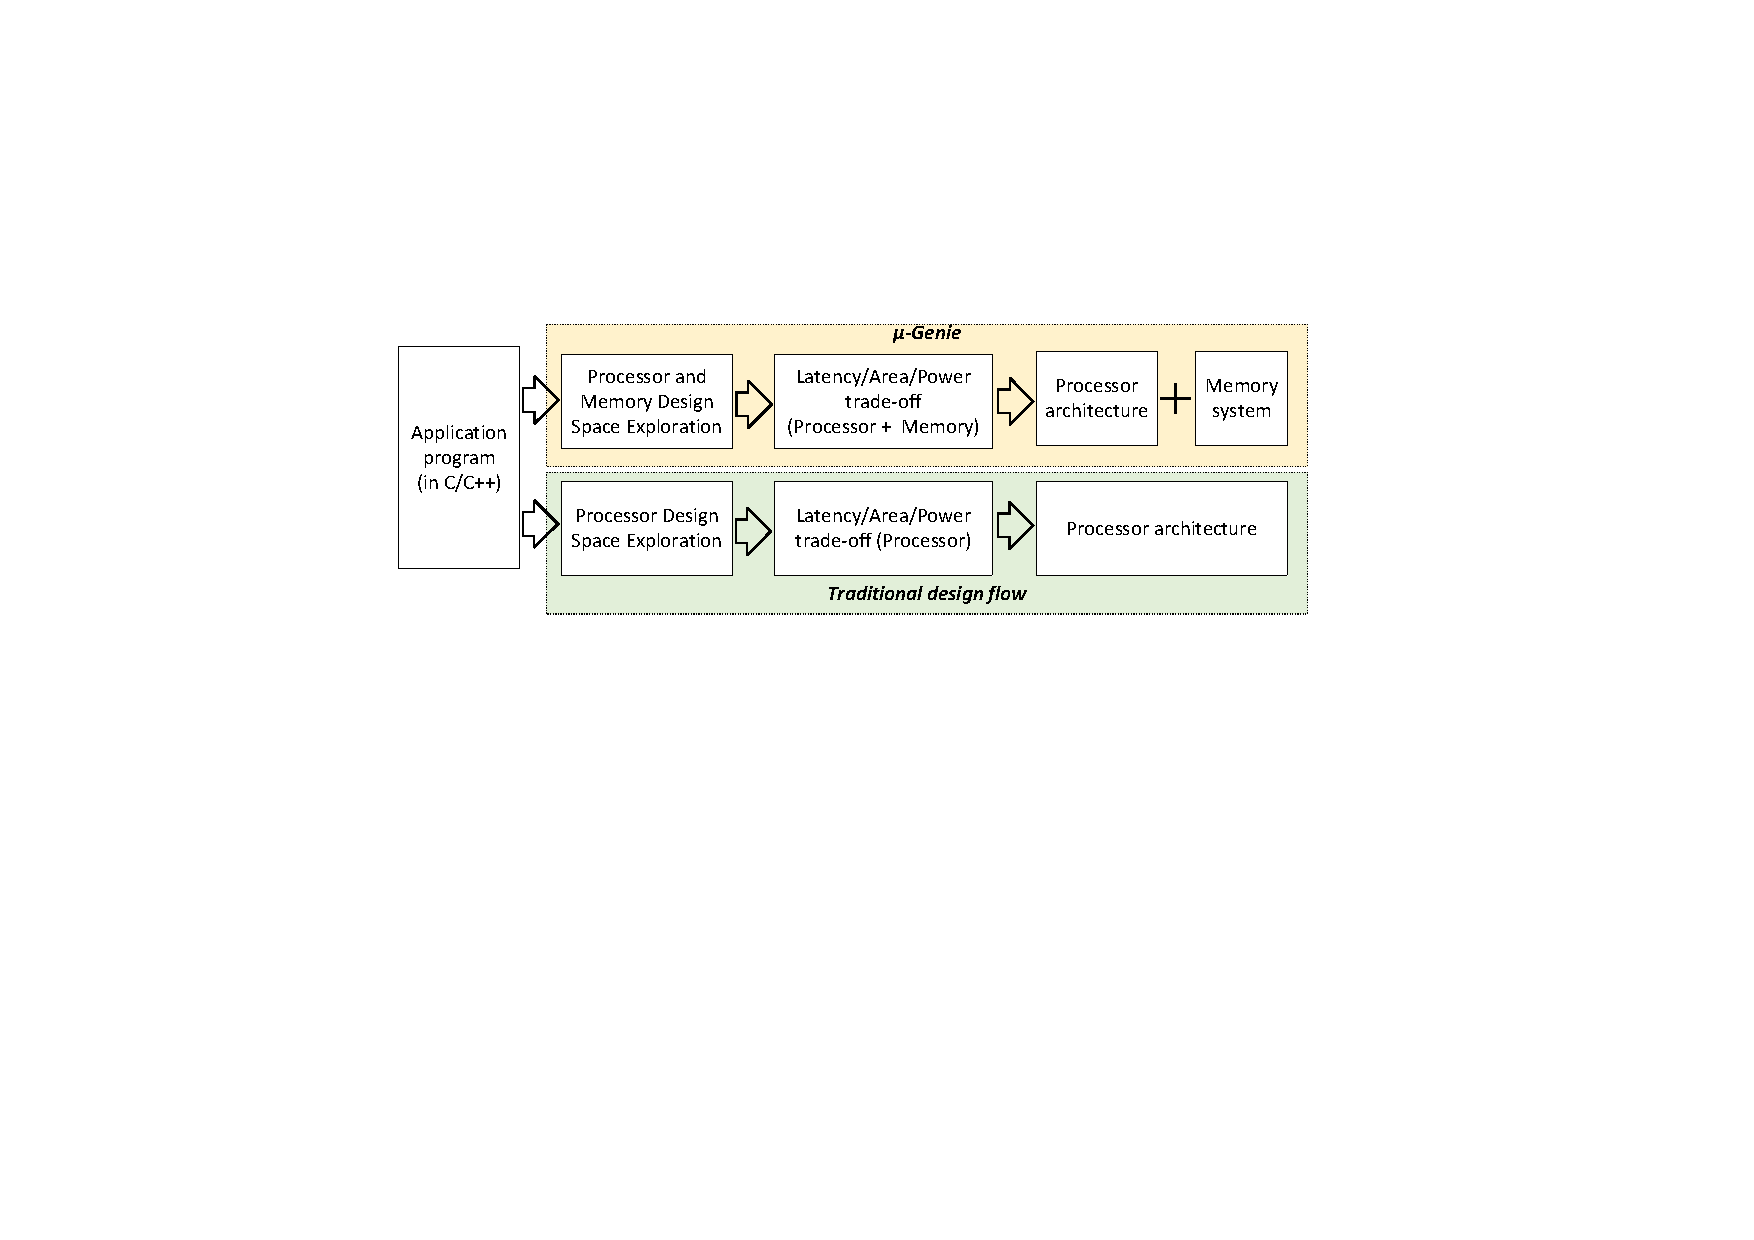
\includegraphics[clip, trim=6cm 10.5cm 6.4cm 5.2cm, width=1.0\linewidth]{images/intro_figure.pdf} %[left down right up ] 
    \caption{Difference between state-of-the-art and the proposed \frameworkname~design flow custom processor architecture design and implementation.}
    \label{fig:intro}
\end{figure}

With the massive increase in the data handling needed in custom hardware, the memory system (both on-chip and off-chip) is becoming a dominant factor in terms of performance, power consumption and area usage. Since the memory system and the processing system are \textit{interdependent}, they should be \textit{co-designed}. This is especially important while using emerging memory technologies with different access latencies for read and write operations but offers high integration density and often low power than SRAM.

Our main contributions in this paper are:
\begin{itemize}
\item \frameworkname: An automated framework for memory-aware custom processor architecture design-space exploration and provide different area/latency tradeoffs, as shown in Figure~\ref{fig:intro}. The framework allows use of different kind of memory technologies and configuration of different parameters such as, levels of memory, clock speed, read/write latency and data width. 
\item A novel spatial processor architecture template that can be configured at design-time and allows a faster implementation of an application-specific hardware.
\item Case-study demonstrating the effectiveness of the framework for a custom processor design using state-of-the-art MRAM and SRAM for memory system.


%In this work we present \frameworkname, a framework that allows to compare design choices and perform automatic system level design and implementation. We propose a novel memory-driven approach for application-specific hardware design starting from two observations. First, the memory system and the processing system are \textit{interdependent} and therefore they should be \textit{co-designed}. Second, the \textit{data dependencies} of the fixed application impose constaints on the design of both memory and processing systems. Hence, our approach starts from the analysis of an input application and codesigns memory and custom processor, shown in Figure~\ref{fig:intro}. 


\end{itemize}


The rest of this paper is organized as follows. We ..

